\section{eo\-NDSorting\_\-II$<$ EOT $>$ Class Template Reference}
\label{classeo_n_d_sorting___i_i}\index{eoNDSorting_II@{eoNDSorting\_\-II}}
Fast Elitist Non-Dominant Sorting Genetic Algorithm.  


{\tt \#include $<$eo\-NDSorting.h$>$}

Inheritance diagram for eo\-NDSorting\_\-II$<$ EOT $>$::\begin{figure}[H]
\begin{center}
\leavevmode
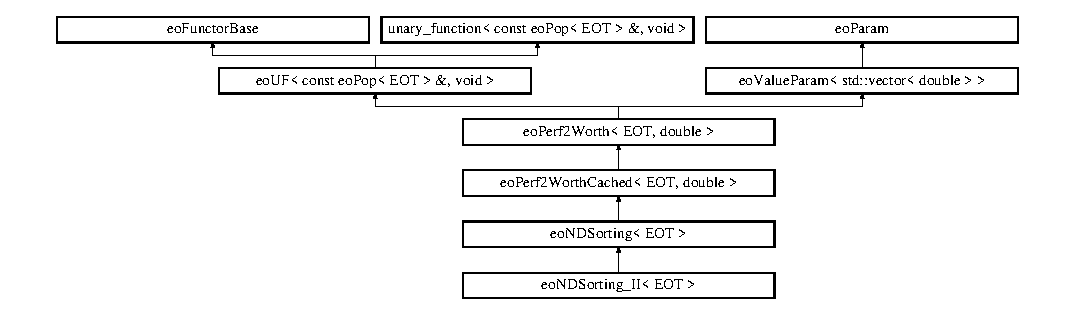
\includegraphics[height=3.78378cm]{classeo_n_d_sorting___i_i}
\end{center}
\end{figure}
\subsection*{Public Types}
\begin{CompactItemize}
\item 
typedef std::pair$<$ double, unsigned $>$ {\bf double\_\-index\_\-pair}\label{classeo_n_d_sorting___i_i_w0}

\end{CompactItemize}
\subsection*{Public Member Functions}
\begin{CompactItemize}
\item 
{\bf eo\-NDSorting\_\-II} (bool nasty\_\-flag\_\-=false)\label{classeo_n_d_sorting___i_i_a0}

\item 
std::vector$<$ double $>$ {\bf niche\_\-penalty} (const std::vector$<$ unsigned $>$ \&\_\-cf, const {\bf eo\-Pop}$<$ {\bf EOT} $>$ \&\_\-pop)\label{classeo_n_d_sorting___i_i_a1}

\begin{CompactList}\small\item\em \_\-cf points into the elements that consist of the current front \item\end{CompactList}\end{CompactItemize}


\subsection{Detailed Description}
\subsubsection*{template$<$class EOT$>$ class eo\-NDSorting\_\-II$<$ EOT $>$}

Fast Elitist Non-Dominant Sorting Genetic Algorithm. 

Adapted from Deb, Agrawal, Pratab and Meyarivan: A Fast Elitist Non-Dominant Sorting Genetic Algorithm for Multi\-Objective Optimization: NSGA-II Kan\-GAL Report No. 200001

Note that this class does not do the sorting per se, but the sorting of it worth\_\-std::vector will give the right order

The crowding distance is calculated as the sum of the distances to the nearest neighbours. As we need to return the penalty value, we have to invert that and invert it again in the base class, but such is life, sigh 



Definition at line 434 of file eo\-NDSorting.h.

The documentation for this class was generated from the following file:\begin{CompactItemize}
\item 
eo\-NDSorting.h\end{CompactItemize}
